\documentclass{article}
\usepackage{import}
\usepackage[utf8]{inputenc}
\usepackage{amsmath}
\usepackage{amssymb}
\usepackage{mathtools}
\usepackage{graphicx}
\usepackage{tabularx}
\usepackage{float}
\usepackage{subfig}
\usepackage{lscape} 
\usepackage{hyperref}
\usepackage{setspace}
\usepackage{booktabs}
\usepackage[authoryear]{natbib}
\usepackage{lmodern}
\usepackage[T1]{fontenc}
\usepackage[bottom]{footmisc}
\newcommand{\indep}{\perp \!\!\! \perp}
\usepackage[nolist]{acronym}
\newcommand\headercell[1]{%
   \smash[b]{\begin{tabular}[t]{@{}c@{}} #1 \end{tabular}}}
\usepackage[a4paper,top=3cm,bottom=2cm,left=3cm,right=3cm,marginparwidth=1.75cm]{geometry}
\usepackage{xcolor}%
\definecolor{webbrown}{rgb}{.6,0,0}
\usepackage{hyperref}%
\hypersetup{%
  breaklinks = true,%
  colorlinks = true,%
  anchorcolor = webbrown,%
  citecolor = webbrown,%
  filecolor = webbrown,%
  linkcolor = webbrown,%
  menucolor = webbrown,%
  urlcolor= webbrown,%
  citebordercolor= 1 0 0,%
  menubordercolor=1 0 0,%
  urlbordercolor=1 0 0,%
  runbordercolor=1 0 0,}
\usepackage{cleveref}

\usepackage{setspace}
\usepackage{enumitem}
\setstretch{1.5} %% set line spacing

\begin{acronym}
  \acro{CI}{confidence interval}
  \acro{RCT}{randomized controlled trial}
  \acro{IV}{instrumental variable}
  \acro{LATE}{local average treatment effect}
  \acro{ATE}{average treatment effect}
  \acro{OLS}{ordinary least squares}
  \acro{RD}{regression discontinuity}
  \acro{MTE}{marginal treatment effect}
  \acro{ATT}{average treatment effect on the treated}
\end{acronym}

\graphicspath{ {../../output/figures/} }

% Wrap table notes
\usepackage{booktabs}
\newcommand{\tabnotes}[2]{\bottomrule \multicolumn{#1}{@{}p{0.70\linewidth}@{}}{\footnotesize #2 }\end{tabular}\end{table}}

\floatplacement{figure}{H}
\floatplacement{table}{H}

\usepackage[toc,page]{appendix}


\title{TITLE:\texorpdfstring{\\}{} subtitle}
\author{Ray Huang\thanks{Contact:
    \href{mailto:ray_huang@brown.edu}{ray\_huang@brown.edu}.
     I thank Peter Hull at Brown University for serving as my advisor and for providing me with fantastic feedback.}
     \\Brown University, Honors Thesis}

\date{\today}

\begin{document}

\maketitle

\begin{abstract}
\noindent Aspirational abstract goes here!
\end{abstract}

\clearpage

\section*{Introduction}

\section*{Motivation and Background}

\section*{Data Description}


\section*{Empirical/Econometric Methods, Hypotheses tested}

\section*{Figures}

\begin{center}
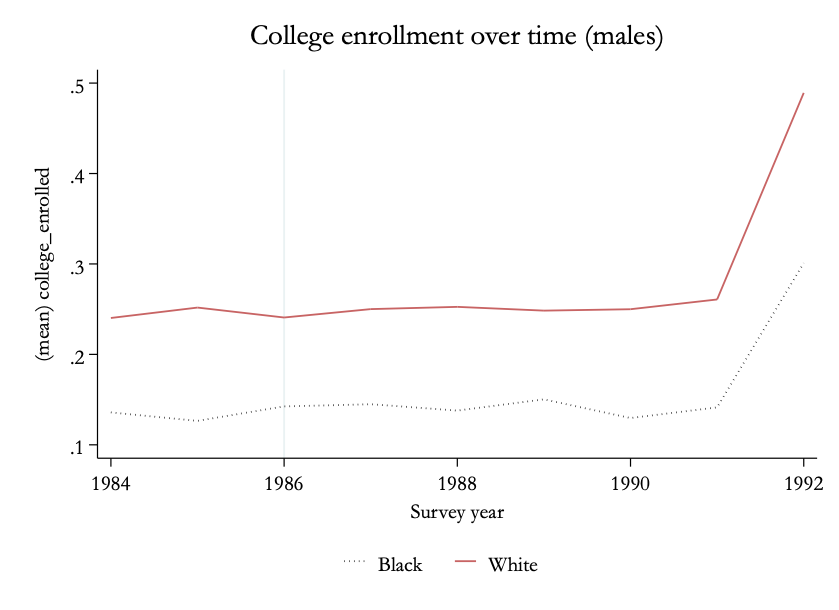
\includegraphics[width=.4\textwidth]{college_enroll_byrace_1986.png}
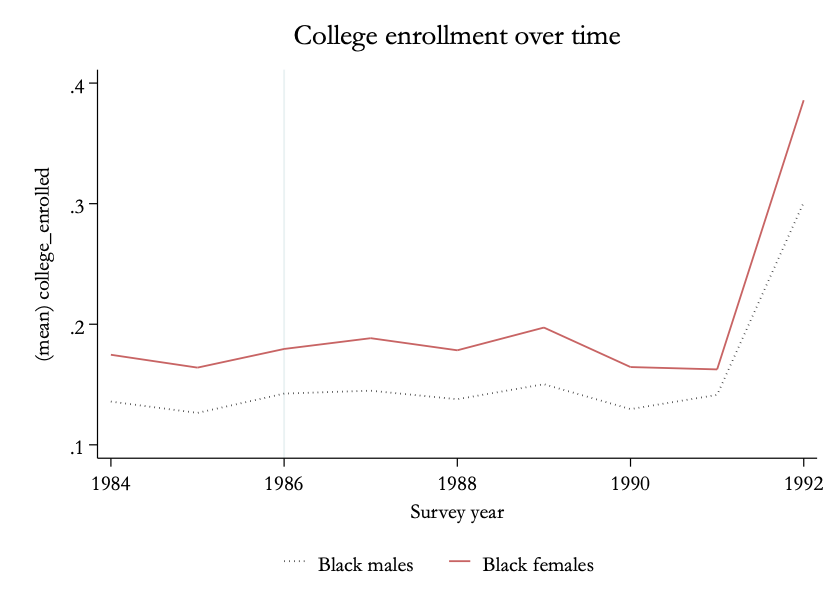
\includegraphics[width=.4\textwidth]{college_enroll_bysex_1986.png}
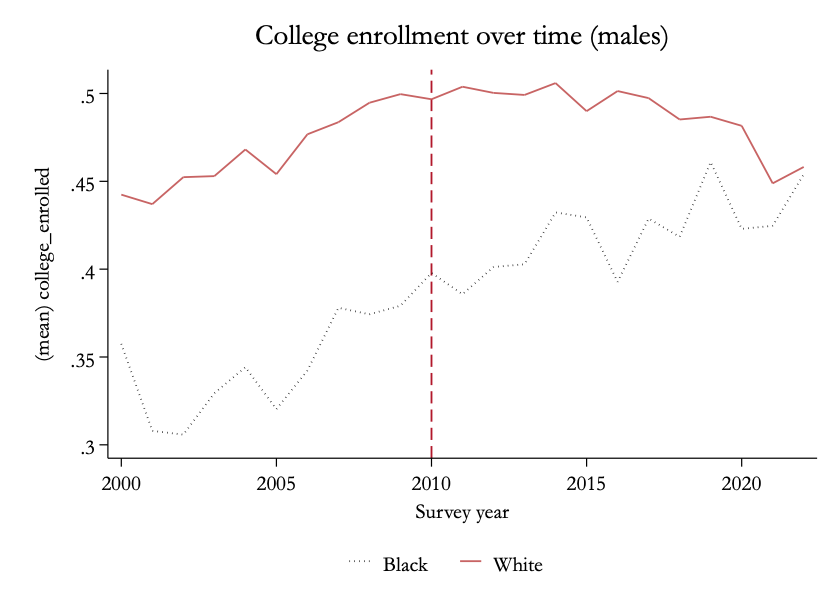
\includegraphics[width=.4\textwidth]{college_enroll_byrace_2010.png}
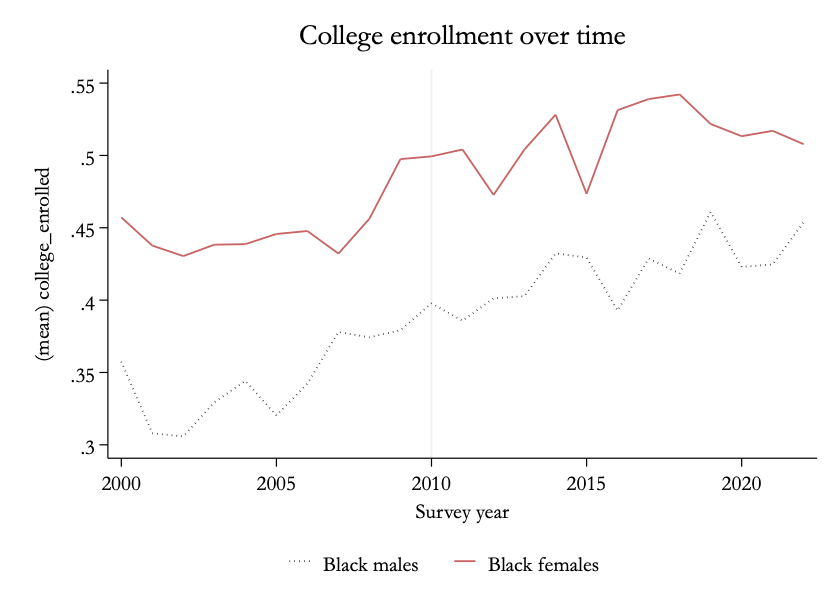
\includegraphics[width=.4\textwidth]{college_enroll_bysex_2010.png}
\end{center}


\section*{Tables}
\import{../../output/tables/}{britton_summ_stats.tex}

\import{../../output/tables/}{britton_table2_DiD.tex}

\import{../../output/tables/}{britton_table3_DiD.tex}

\import{../../output/tables/}{fair_sentencing_DiD_t1.tex}

\import{../../output/tables/}{fair_sentencing_DiD_t2.tex}



%%%%%%%%%%%%%%%%%%%%%%%%BIB%%%%%%%%%%%%%%%%%%%%%%%%%%%

\clearpage
\nocite{*}
\singlespacing
\bibliographystyle{jpe}
\bibliography{citations.bib}

%%%%%%%%%%%%%%%%%%%%%%%%FIGURES%%%%%%%%%%%%%%%%%%%%%%%%%%%

\clearpage

\end{document}
